\documentclass[../../doc.tex]{subfiles}
\graphicspath{{\subfix{../../img}}}
\begin{document}
    \subsection{Уравнение динамики}

    Для получения уравнения динамики рассматриваемой физической системы воспользуемся методом Эйлера--Лагранжа \cite{kolubin2017}.
    Идея метода состоит в проведении следующих последовательных шагов:
    \begin{enumerate}\itemsep0em 
        \item Выбор обобщенных координат;
        \item Получение выражения для кинетической $K$ и потенциальной $\Pi$ энергий системы, записанных в обобщенных координатах;
        \item Получение выражения для лагражиана системы $\mathcal{L}$;
        \item Составление системы уравнений движения, соответствующих каждой обобщенной координате.
    \end{enumerate}

    Обобщенными координатами для нашей системы выберем углы поворота сочленений $\theta_i$, $i = 1, 2, 3$.
    Далее перейдем к выражению энергий через обобщенные координаты.

    Для подсчета кинетической энергии воспользуемся теоремой Кёнинга~[ссылка куда-то].
    \begin{theorem}[Кёнинг]
        Кинетическая энергия тела есть энергия поступательного движения центра масс плюс энергия вращательного движения относительно центра масс
        \begin{equation}\label{eq:kin-energy}
            K = \frac{1}{2} m \|v_c\|^2 + \frac{1}{2}\omega^{\T} I \omega,
        \end{equation}
        где $m$~--- полная масса тела, $I$~--- тензор инерции тела, $v_c$~--- линейная скорость центра масс, $\omega$~--- скорость вращения тела относительно центра масс.
    \end{theorem}

    Далее в работе мы будем полагать, что каждое из сочленений представляет собой однородный стержень длины $l_i$ массы $m_i$.
    В таком случае получаем следующие значения для положения центра масс~$c^i \in \mathbb{R}^2$ $i$-ого сочленения:
    $$
        c^i =
        \left[\begin{aligned}
            \sum_{j=1}^{i-1} l_j cos\theta_j + \frac{l_i}{2}cos\theta_i \\
            \sum_{j=1}^{i-1} l_j sin\theta_j + \frac{l_i}{2}sin\theta_i
        \end{aligned}\right].
    $$
    Выражения для момента инерции и скорости вращательного движения относительно центра масс для стержня получаются соответственно:
    $$
        I_i = \uint\limits_{(m_i)} r^2\,dm = \rho_i\uint\limits_{(l_i)} r^2\,dl = \frac{m_il_i^2}{12},
    $$
    $$
        \omega_i = 2\dot \theta_i.
    $$
    Потенциальная энергия $i$-ого сочленения рассчитывается по формуле
    $$
        \Pi_i = m_i g c^i_2,
    $$
    где $g \approx 9,\!8$~--- ускорение свободного падения.

    Общая кинетическая и потенциальная энергии системы рассчитываются как сумма энергий каждого из сочленений:
    $$
        K = \sum_{i=1}^{3} K_i = \sum_{i=1}^{3}\left( \frac{m_i \|\dot c^i\|^2}{2} + \frac{m_i l_i^2 |\dot \theta_i|^2}{6} \right),
    $$
    $$
        \Pi = \sum_{i=1}^{3} \Pi_i = \sum_{i=1}^{3} m_i g c^i_2.
    $$

    Теперь введём лагражиан системы
    $$
        \mathcal{L} = K - \Pi
    $$
    и построим систему уравнений Эйлера--Лагранжа~[ссылка]:
    \begin{equation}\label{eq:euler-lagrange}
        \frac{d}{dt} \frac{\partial \mathcal{L}}{\partial \dot \theta_i} - \frac{\partial \mathcal{L}}{\partial \theta_i} = \tau_i,\; i = \overline{1, 3},
    \end{equation}
    где $\tau_i$~--- момент силы, действующий на $i$-ое сочленение, который доступен для управления.

    Продифференцировав члены из левой части уравнения \eqref{eq:euler-lagrange}, получим уравнение динамики для рассматриваемой системы:
    \begin{equation}\label{eq:dynamic}
        M(\theta)\ddot\theta + L(\theta, \dot\theta) = \tau,
    \end{equation}
    где $M(\theta) = M \T (\theta) \in \mathbb{R}^{3 \times 3}$~--- матрица инерции системы, $L(\theta, \dot\theta)\in\mathbb{R}^{3}$~--- вектор центростремительных и кореолисовых сил.
    На Рис.~\ref{img:pendulum} приведено численное моделирование свободного падения в соответствии с полученным уравнением динамики~\eqref{eq:dynamic}.

    \begin{remark}
        Матрица инерции $M(\theta)$ является положительно-опре\-де\-лён\-ной, поскольку кинетическая энергия системы~$K$ всегда неотрицательна:
        \begin{equation*}
            K(\theta, \dot\theta) = \frac{1}{2}\left\langle \dot \theta, M(\theta) \dot \theta \right\rangle > 0 \mbox{ для любого } \dot \theta \neq 0.
        \end{equation*}
    \end{remark}

    \begin{figure}[h]
        \begin{center}
            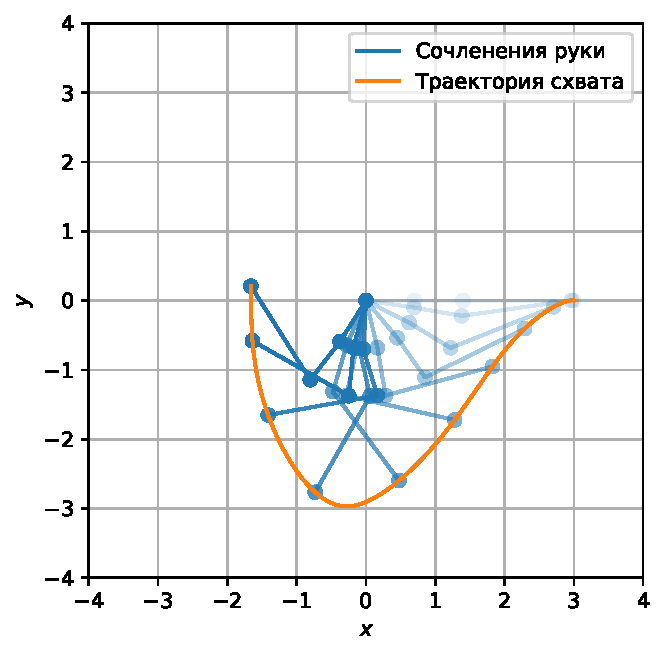
\includegraphics[width=0.5\textwidth]{model/pendulum}
        \end{center}
        \caption{
            Траектория руки $l = [0,\!7\; 0,\!7\; 1,\!6]\T$, $m = [0,\!8\; 0,\!8\; 1,\!2]\T$ в свободном падении из начального положения $\theta^{\textnormal{start}} = [0\; 0\; 0]\T$, $\dot\theta^{\textnormal{start}} = [0\;0\;0]\T$ на временном интервале $0 \leqslant t \leqslant 1$.
            Положения, соответствующие более раннему времени, показаны бледнее.
            Всюду далее работе для численного моделирования используется данная конфигурация маятника $l$, $m$.
        }
        \label{img:pendulum}
    \end{figure}

    \ifSubfilesClassLoaded{
        \nocite{*}
        \clearpage
        \bibliographystyle{plain}
        \bibliography{../../refs}
    }{}
\end{document}